\chapter[Proposta]{Proposta}

A proposta deste trabalho foi a construção de um \textit{framework} de definição de trajetória para robôs móveis, mais especificamente, algoritmos globais de definição de trajetória. Foi implementado os quatro algoritmos descritos no capítulo 2 (Grafo de Visibilidade, Voronoi, Quadtree e Wavefront). Um mapa do ambiente é recebido da camada de mapeamento e o algoritmo cria um grafo a partir dele, definindo os caminhos livres que podem ser percorridos. Após isso é rodado um algoritmo de melhor caminho (como Djikstra por exemplo) para definir o caminho a ser percorrido pelo robô. 

A Figura 19 demonstra as tarefas principais do \textit{framework}, bem como suas entradas e saídas. Essas entradas e saídas definem como ele se comunica com as demais camadas do robô e as dependências dele para cumprir seu funcionamento. Cada tarefa apresentada representa um módulo do \textit{framework} e as interações entre eles as estruturas de dados utilizadas para se comunicarem.
 
\begin{figure}[h]
	\centering
	\label{fig19}
		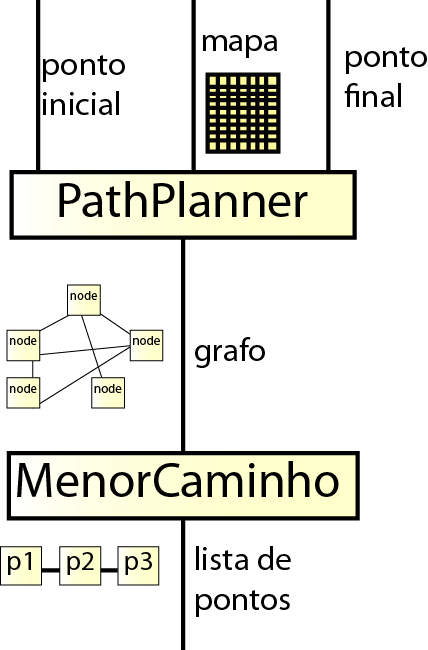
\includegraphics[keepaspectratio=true,scale=1]{figuras/framework.png}
	\caption{estrutura do funcionamento do \textit{framework}}
\end{figure} 

A arquitetura geral do robô foi considerada como na Figura 20 apresentada por \cite{Nehmzow2003}. Todas as abordagens da arquitetura de navegação seguiam uma lógica semelhante e apresentavam pequenas diferenças entre si. Assim sendo, esta estrutura mantêm as características apresentadas no capítulo 2.

\begin{figure}[h]
	\centering
	\label{fig20}
		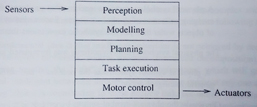
\includegraphics[keepaspectratio=true,scale=1]{figuras/arqusada.jpg}
	\caption{arquitetura a navegação considerada, \cite{Nehmzow2003}}
\end{figure}

A definição de trajetória e o \textit{framework} participam da terceira camada. Como as camadas acima são responsáveis pelo mapeamento e entregam o mapa completo, os algoritmos globais e este \textit{framework} não precisam se preocupar com comunicação com os sensores. As camadas abaixo recebem a lista de coordenadas para onde deve ir e cuidam do controle dos motores para chegar neles considerando os graus de liberdade do robô (que varia de acordo com sua estrutura física). Assim, a camada a ser criada não se comunica nem com os sensores nem com os motores, o que lhe dá maior independência das configurações de robô. Com isso é esperado que o \textit{framework} funcione em variados tipos de robôs, não apenas no modelo \textit{differential steering} testado.

A seguir é definido como funciona os detalhes do \textit{framework} levantados no capítulo 2.

\section{A arquitetura}

A arquitetura de navegação costuma ser em camadas, como mostrado no capítulo 2. Este \textit{framework} trabalha dentro da camada de planejamento de trajetória e é uma estrutura baseada em componentes. Uma arquitetura em camadas dentro de outra poderia gerar indireções desnecessárias, além de uma abordagem por componentes suprir melhor as necessidades do \textit{framework}.

Cada funcionalidade é efetuada por um componente diferente, projetado para consumir o mínimo de memória e depender o mínimo de outros componentes e de bibliotecas externas (incluindo as próprias do Java). Cada módulo tem a preocupação de ser o mais auto-suficiente possível, tendo apenas as interações necessárias para o seu funcionamento. Cada um dos módulos será constantemente avaliado quando a seu acoplamento, coesão,  simplicidade e facilidade de compreensão. Estas características serão melhor definidas na seção 4.5.

O \textit{framework} segue o padrão caixa-cinza, pois é desejável que o mesmo seja transparente e configurável pelo usuário. O usuário do \textit{framework} é livre para usar as implementações já prontas dos algoritmos de definição de trajetória e melhor caminho ou criar as suas próprias a partir das classes abstratas fornecidas. Além disso o fluxo de execução e alguns comportamentos são mantidos estáticos.

O diagrama de componentes da Figura 21 mostra os módulos do sistema e suas interações. Nele mostramos os componentes conhecidos por cada outro componente, mas não quais classes. Levando em conta o princípio de programar para interfaces, as classes conhecidas serão sempre as interfaces e classes abstratas (exceto nos compententes de estrutra de dados). Para simplificar o diagrama, as classes concretas foram retiradas e criado um diagrama para detalhar cada módulo.

\begin{figure}[h]
	\centering
	\label{fig21}
		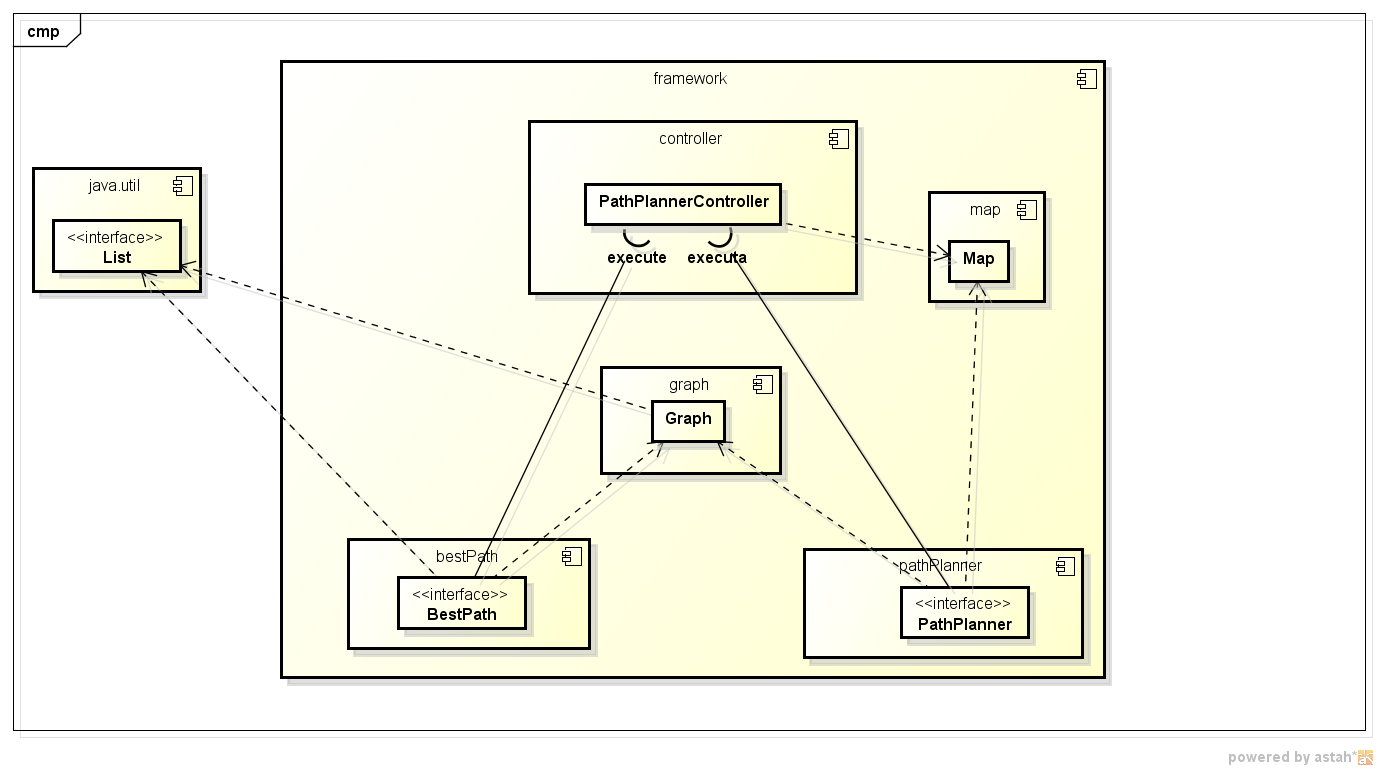
\includegraphics[keepaspectratio=true,scale=0.4]{figuras/componentes.png}
	\caption{diagrama de pacotes do sistema}
\end{figure}

A seguir cada componente é descrito mais detalhadamente e são abordadas suas classes abstratas e concretas.

\subsection{Controller}

\begin{figure}[h]
	\centering
	\label{fig22}
		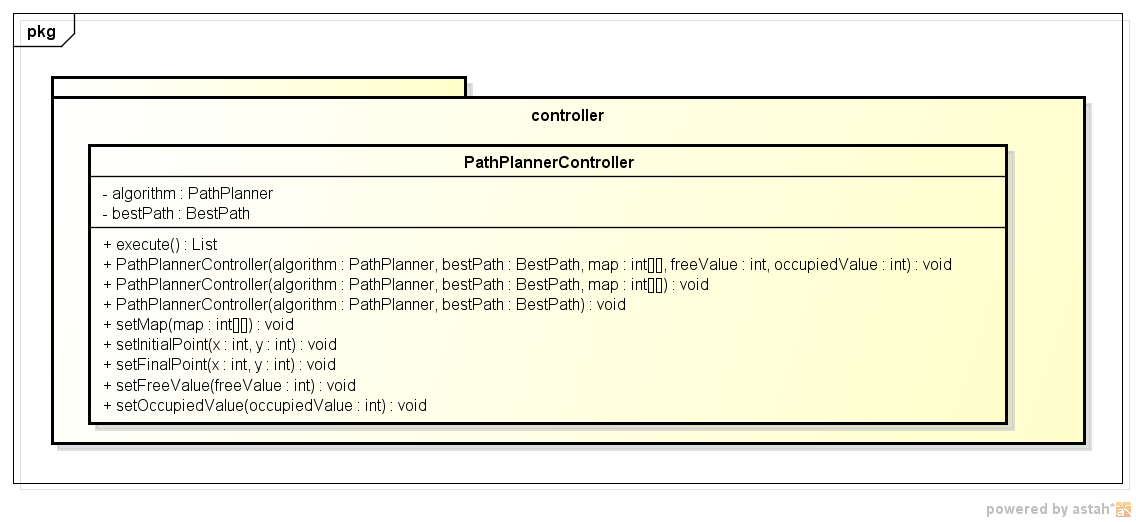
\includegraphics[keepaspectratio=true,scale=0.5]{figuras/pkgcontroller.png}
	\caption{componente Controller}
\end{figure}

A classe PathPlannerController tem como propósito servir de intermediário entre o usuário do \textit{framework} e as funções implementadas por ele. Ela controla o fluxo de trabalho da aplicação, chamando os métodos das demais classes na ordem e verificando seu correto funcionamento.

O componente segue os princípios Controlador e Inversão de Controle. Em vez do usuário chamar todas as funções do componente e fazer seu controle diretamente toda vez que quiser definir uma trajetória, este componente realiza esta tarefa por ele, diminuindo acoplamento entre o usuário e o subsistema. A Inversão de Controle está presente pelo usuário não ser o responsável por instanciar as classes do outros componentes. Embora o \textit{framework} as use, cabe ao usuáio instanciá-las e definir quais de suas variações será implementada. No construtor da classe é passado os objetos PathPlanner e BestPath, que são armazenados e usados no método \textit{execute} para realizar o cálculo do percurso. Isso permite ao módulo não conhecer as variações de cada interface, desacoplando-o dos demais módulos.

Os padrões utilizados são o Fachada e a Injeção de Dependência.

É também atribuído a esse módulo a responsabilidade por criar a estrutura local do mapa. O controlador o inicializa e define os pontos iniciais e finais, além de limpá-lo das alterações feitas ao final, deixando ao componente PathPlanner apenas a tarefa de utilizá-lo.

O diagrama de sequência apresentado na seção 2.4 mostra de forma bastante superficial o funcionamento do sistema para dar uma visão geral das funcionalidades e sequência de ações. O diagrama na Figura 23 demonstra de forma mais aprofundada como realmente é feito o trabalho do framework, com foco no componente controller.

\begin{figure}[h]
	\centering
	\label{fig23}
		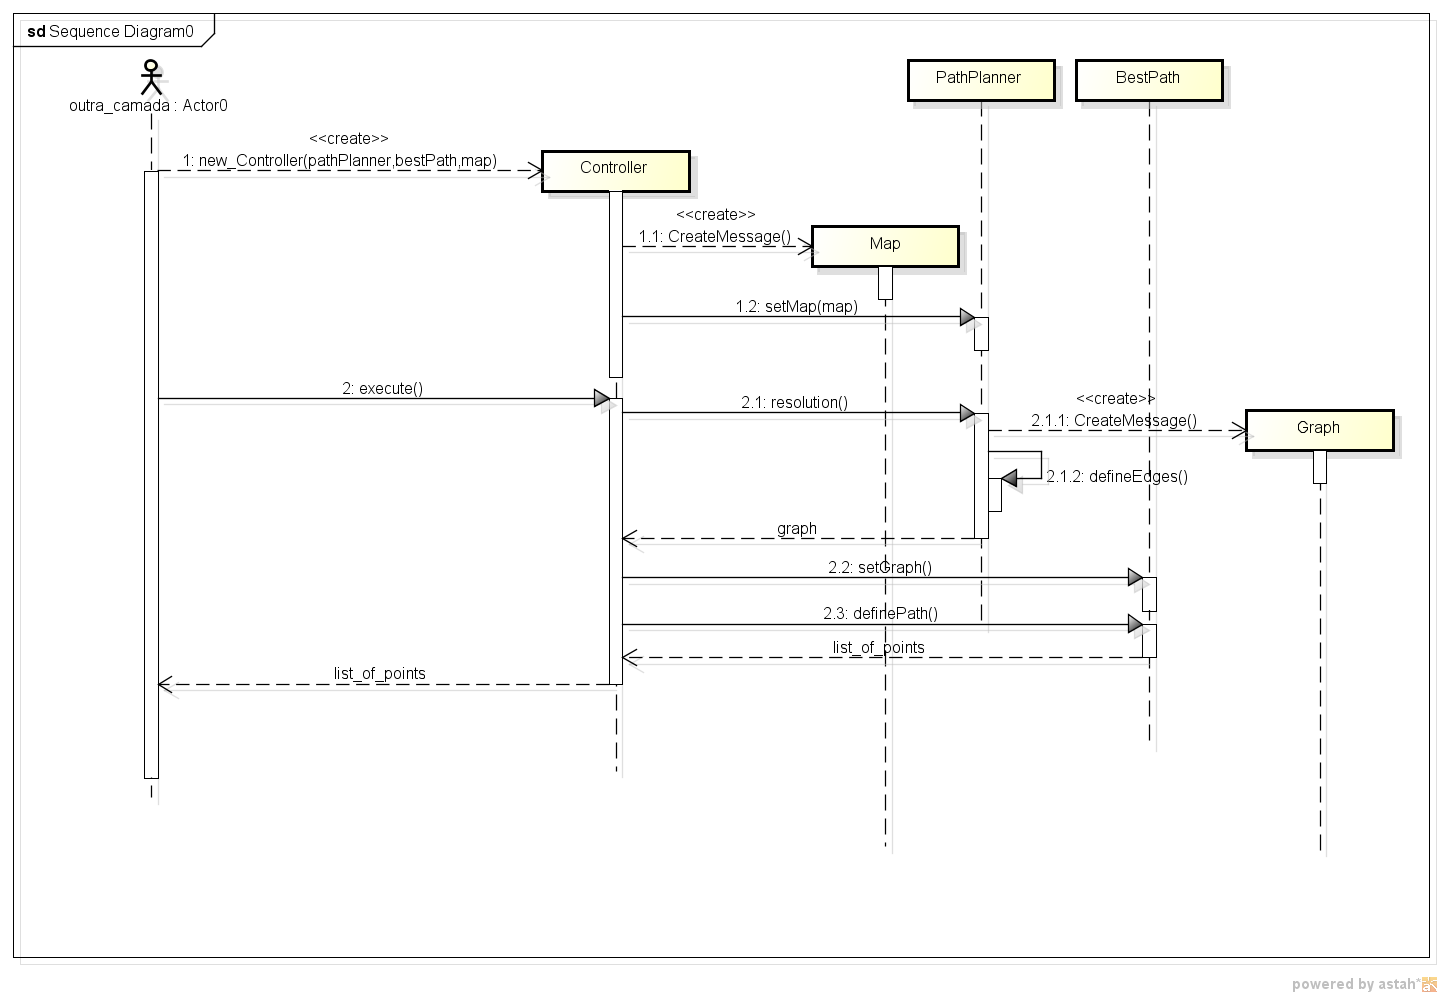
\includegraphics[keepaspectratio=true,scale=0.4]{figuras/executeController.png}
	\caption{diagrama de sequência do componente controller}
\end{figure}

\subsection{Map}

\begin{figure}[h]
	\centering
	\label{fig24}
		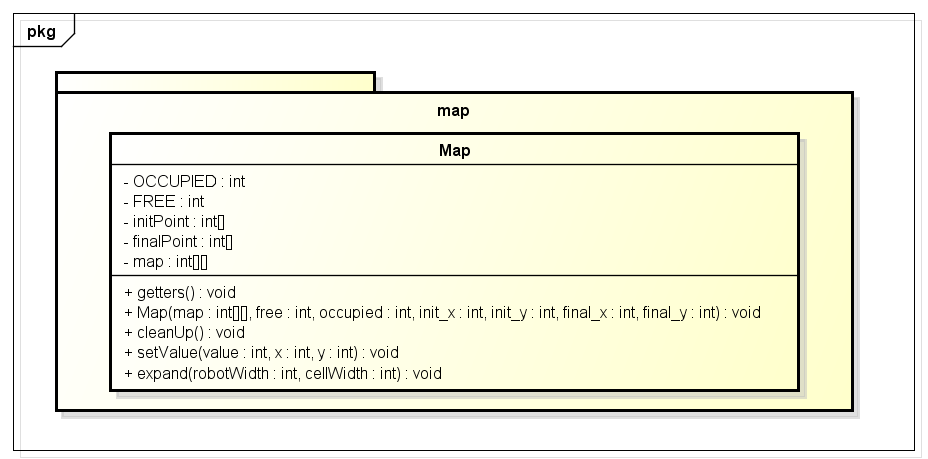
\includegraphics[keepaspectratio=true,scale=0.5]{figuras/pkgmap.png}
	\caption{componente Map}
\end{figure}

O componente Map armazena a estrutura do mapa em seu interior. O componente recebe do controlador os dados das posições e guarda essa referência dentro de si para fazer as alterações necessárias. O objeto Map centraliza os dados que a camada de sensoriamento fornece e funções específicas da definição de trajetória que age sobre eles, como definir ponto inicial, final, dar pesos as posições (células), expandir obstáculos e diferenciar espaço livre de obstáculos. No final, para não invalidar os dados da camada de mapeamento, as alterações feitas são desfeitas por esta classe com a função \textit{cleanUp}.

Para proteger os dados do mapa, seus valores são todos passados via construtor e disponibilizado apenas os métodos \textit{get}. Isso evita que novos pontos iniciais e finais sejam inclusos ou alterados. A única exceção são as posições livres, que podem receber pesos no algoritmo Wavefront e precisam ser alteradas.

\subsection{Path Planner}

\begin{figure}[h]
	\centering
	\label{fig25}
		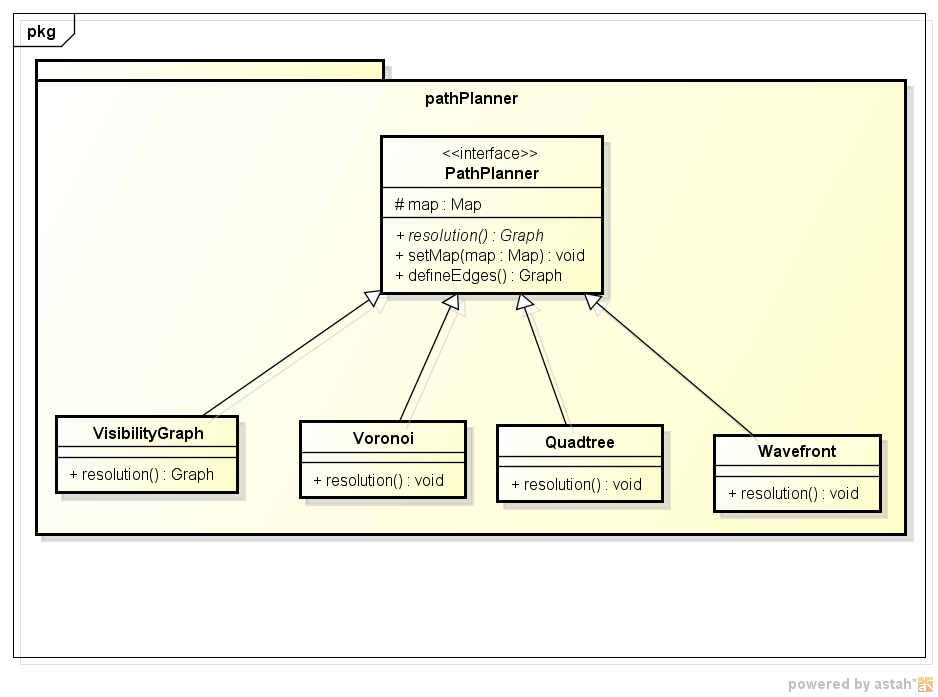
\includegraphics[keepaspectratio=true,scale=0.5]{figuras/pkgpathplanner.png}
	\caption{componente PathPlanner}
\end{figure}

O PathPlanner é o componente responsável por implementar os algoritmos de definição de trajetória. A classe abstrata PathPlanner carrega funções úteis às classes concretas e fornece um método abstrato que deve realizar o algoritmo. Cada subclasse implementa \textit{resolution} e métodos específicos e cria um grafo diferente.

Graças à interface comum aos algoritmos é possível tratá-los de forma igual em todo o resto do sistema. O comportamento diferente entre eles (a criação do grafo) é abstraído para as subclasses enquanto a superclasse implementa o que for igual e define as entradas e saídas comuns a todos eles. Isso segue o princípio de Variações Protegidas apresentado por \cite{Larman2005}, implementado através do padrão Strategy. O padrão Injeção de Dependência diminui seu acoplamento com o módulo Map, recebendo o mapa já pronto para trabalhar do controlador.

\subsection{Graph}

\begin{figure}[h]
	\centering
	\label{fig26}
		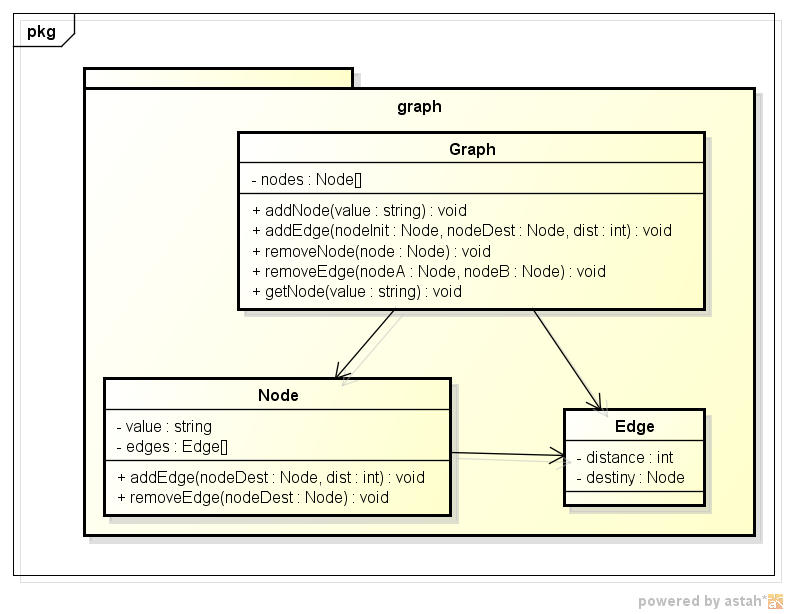
\includegraphics[keepaspectratio=true,scale=0.5]{figuras/pkggraph.png}
	\caption{componente Graph}
\end{figure}

O módulo Graph é responsável por manter a estrutura do grafo. O grafo mantém uma lista de nós que representam pontos navegáveis no espaço. Cada nó possui uma lista de arestas (\textit{edges}) que o liga a outros nós.

A classe grafo possui métodos para a construção, busca e eliminação de nós e arestas, podendo realizar qualquer operação CRUD através do próprio objeto grafo ao invés de trabalhar diretamente em cada nó.

\subsection{Best Path}

\begin{figure}[h]
	\centering
	\label{fig27}
		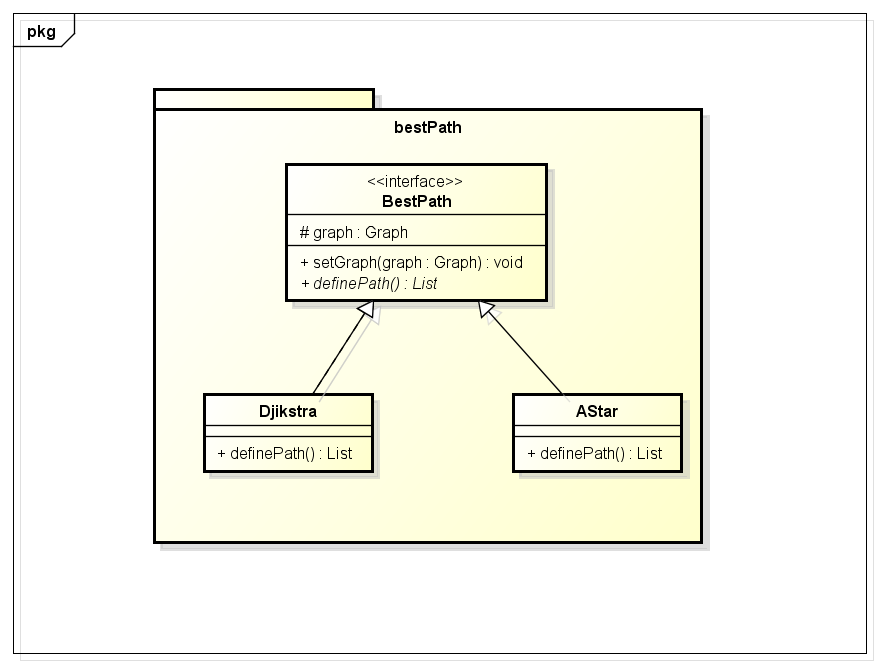
\includegraphics[keepaspectratio=true,scale=0.5]{figuras/pkgbestPath.png}
	\caption{componente BestPath}
\end{figure}

O Best Path é o componente que define o melhor caminho a ser executado pelo robô. Recebendo o grafo com os pontos navegáveis, este módulo define um trajeto a partir de alguma característica desejada (menor caminho, menor curvatura...). Esta carecterística é definida pela subclasse escolhida pelo usuário. No caso, as duas subclasses mostradas no diagrama definem o percurso por menor caminho, porém novas extensões podem ser criadas para formar o trajeto a partir de outra característica.

Novamente, a classe abstrata BestPath define as características comuns a todos os algoritmos, determinando as entradas e saídas que receberão. A implementaçao de como trabalhar com o grafo e criar a lista de pontos pelos quais o robô passará dependerá da implementação escolhida.

Assim como no componente pathPlanner, o princípio de Variações Protegidas é realizado através do padrão Strategy.

\section{O mapa}

Todo o processo se inicia com o recebimento do mapa para então operar sobre o mesmo. Dentre os tipos de estrutras de dados que representa o mapa citados no capítulo 2 o esperado pelo \textit{framework} será uma malha de ocupação. Junto com a matriz será recebido os valores para terreno ocupado e livre. A seguir deve ser marcado no mapa quais são os pontos iniciais e finais.

O \textit{framework} usa uma estrutura própria para armazenar estes dados, porém guarda referência aos dados originais da camada de sensoriamento, evitando o gasto excessivo de memória para a mesma informação. As alterações nos dados do mapa deverão ser revertidas ao fim do processamento do \textit{framework}, devolvendo ao mapa seus dados originais.

\section{Os obstáculos}

Os obstáculos são representados por células de valores diferentes no mapa, marcando-as como ocupadas. Contudo algumas considerações sobre os obstáculos precisam ser feitas independente da forma que são implementados.

O robô é considerado como um ponto (seu centro), o que pode gerar problemas se ele se aproximar demais dos obstáculos. Um algoritmo considerando o robô um ponto pode fazê-lo passar muito perto do obstáculo achando que nada acontecerá, porém quando executado o algoritmo o choque ocorre. \cite{Guzman2008} diz que os algorítmos Grafo de Visibilidade e Quadtree passam o mais perto possível dos obstáculos, gerando um menor percurso porém mais perigoso. Para evitar que esses algoritmos causem o choque do robô com o obstáculo uma solução dada por \cite{Souza2008}, \cite{Guzman2008}, \cite{Siegwart2004} e \cite{Thomsen2010} é a expansão dos obstáculos. O algoritmo considera os obstáculos maiores do que realmente são, aumentando o obstáculo em, no mínimo, metade da lagura do robô para que o centro passe tangente ao novo vértice sem haver real contato. Para isso é preciso receber no controlador dois parâmetro a mais, o tamanho do robô e quanto mede cada célula do mapa. O controlador então determina quantas células o robô mede de largura e incrementa a metade mais um em todos os obstáculos.

\begin{figure}[h]
	\centering
	\label{fig28}
		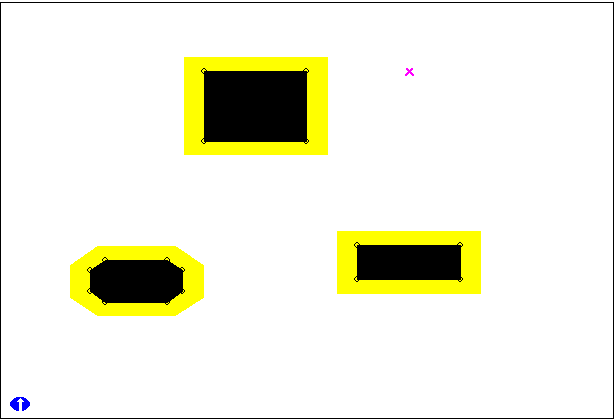
\includegraphics[keepaspectratio=true,scale=0.5]{figuras/expansao.png}
	\caption{obstáculo real em preto e a expansão incrementada em amarelo \cite{MRIT_SITE}}
\end{figure}

Vale lembrar que esta expansão pode mudar o percurso do robô. Um percurso passando entre dois obstáculos pode ser fechado por este incremento. Isso impede que o robô entre em corredores muito estreitos ou entre em regiões côncavas de um obstáculo.

Outra consideração são os obstáculos côncavos. \cite{Siegwart2004} e \cite{Guzman2008} abordam a eliminação de pontos que formem áreas côncavas nos obstáculos. O simulador MRIT citado também segue esta abordagem. Outros autores como \cite{Thomsen2010} e \cite{Choset2005} e  não fazem esta consideração, pois nem sempre o espaço côncavo de um polígono é pequeno a ponto de ser perigoso e por vezes pode ser o único caminho até o objetivo. Considerando que a expansão dos obstáculos já dificulta a chance de choque e que nós que representam um vértice de uma região côncava não serão escolhidos pelos algorítmos e que os espaços côncavos podem ser amplos eles não serão eliminados pelo \textit{framework}.

\section{Hot-spots do framework}

Como definido pelo processo de produção de \textit{framework} de \cite{Fayad1999} a análise de \textit{hot-spots} é algo iterativo, levantado ao longo da produção com apoio de um especialista. Porém, já de início foi realizado uma análise sobre todo o projeto e foram levantados os principais \textit{hot-spots} do sistema. Estes \textit{hot-spots} são o componente \textit{pathPlanner} e \textit{bestPath}. O usuário pode incrementar e configurar estes dois componentes, escolhendo entre as soluções já implementadas e inserindo novas. Suas interfaces servem de gancho para mudanças.

Para dar a variabilidade necessária para a variância destes pontos foi utilizado os padrões de projeto descritos no tópico anterior. Eles oferecem a flexibilidade para mudanças sem gerar impactos nos demais módulos, mantendo a coesão alta e o acoplamento entre os módulos baixo.

\section{Boas práticas de programação}

Não apenas escrever um código que funcione, é preocupação da engenharia de software que o código seja manutenível. Isso inclui, além da modularidade e uso de padrões conhecidos, escrever um código legível e simples. \cite{Goodliffe2007} e \cite{McConnel2004} descrevem características de um bom código e servem como um guia para boa programação.

Essas técnicas dão uma maior qualidade ao código, aumentando manutenibilidade, coesão e reuso. Estes três temas são abordados pelos dois autores. As práticas sugeridas por eles não resolvem os problemas do sistema ou implementam suas funcionalidades, mas estão voltadas para a qualidade a longo prazo. Futuramente, a alteração e inserção de novas funcionalidades ao \textit{framework} será facilitada com estas práticas, permitindo o crescimento do mesmo com menor esforço para sua compreensão.

Algumas dessas características, seguidas no desenvolvimento deste projeto são:

\begin{itemize}
  \item \textbf{Testes inteligentes:} \cite{Goodliffe2007} e \cite{McConnel2004} enfatizam que testes devem ser sempre realizados. Sempre teste o código após fazê-lo, não deixando para outra hora. Eles também enfatizam que os testes devem ser focado nos princiais fluxos do sistema. Tentar testar todas as possibilidades do código é inviável e mutas delas raramente virão a ocorrer. Por isso testes devem ser focados nas partes principais, rodando todos os fluxos das funcionalidades centrais do sistema, testando o \textit{design} do sistema para validá-lo como robusto e testando só os fluxos principais das características menos vitais do sistema. \cite{McConnel2004} sugere o uso de testes automatizados e de cobertura de código.
  \item \textbf{Manter o mesmo estilo de escrita:} o código deve manter o mesmo padrão de escrita por todo o sistema. Se as chaves usadas ao abrir um bloco de instrução estarão na mesma linha ou na de baixo, a identação, comentários, quebras de linha e outras variações devem ser padronizadas para facilitar a leitura e torná-lo mais agradável de ser lido.
  \item \textbf{Nomes significativos:} o leitor deve ser capaz de saber do que se trata a variável, método ou classe apenas lendo seu nome. O nome deve se referir ao comportamento, identidade ou padrão ao qual está relacionado. \cite{Goodliffe2007} afirma que se o programador não sabe qual nome dar a uma variável ou função é porque não sabe exatamente o que ela faz.
  \item \textbf{Testar as entradas do sistema:} Não confiar que os valores recebidos estão sempre corretos é indispensável para um código seguro. Deve-se sempre checar se os valores estão dentro da margem esperada e se objetos não são nulos. Isso vale não só para os dados vindos de fora do \textit{framework}, valores vindo de outras classes e módulos devem ser verificados para garantir que não está sendo recebido um objeto nulo e evitar falhas de segmentação.
  \item \textbf{Clareza sobre código curto:} é preferível que o código fique maior do que difícil de entender. Dividir equações em várias linhas, simplificar as linhas de algorítmos e deixar apenas uma operação por linha são algumas das ações para tornar o código limpo e legível.
  \item \textbf{Considerar casos excepcionais:} mesmo que uma possibilidade de valor seja rara o código deve está preparado para tratá-la. Um conjunto de \textit{if-else-if} em sequência deve sempre ter um bloco \textit{else} ao final para casos fora do esperado, assim como todo bloco \textit{switch} deve possuir uma cláusula \textit{default}. O programa deve estar pronto para criar o objeto incompleto ou lançar algum tipo de exceção nesses casos.
  \item \textbf{Cuidados com variáveis:} sempre inicializar uma variável ao criá-la para evitar ler lixo de memória é uma das ações que tornam o código mais seguro e criar a variável apenas quando ela for útil torna o código mais legível.
  \item \textbf{Evidencie o fluxo padrão do sistema:} O fluxo principal deve ser sempre o primeiro em estruturas condicionais como \textit{if-else} e \textit{switch}. O leitor do código deve conseguir acompanhar o fluxo comum do código sem procurar em uma série de opções nas estruturas condicionais qual é a correta.
  \item \textbf{Simplicidade sobre velocidade:} um código otimizado é mais complexo. Inserir camadas, indireção e linhas extras diminuem a velocidade do sistema, mas o tornam organizado. Serão otimizados apenas blocos de código que necessitem de velocidade. A não ser que seja essencial, deve ser dado prioridade à simplicidade em todo o sistema. Para saber se o código necessita de otimização será preciso testá-lo com uma entrada complexa para analisar o tempo de processamento. Espera-se que os algorítmos Grafo de Visibilidade e Voronoi possam se tornar lentos e, caso isto ocorra de fato, suas implementações serão revistas.
  \item \textbf{Funções atômicas:} cada método deve realizar apenas uma função. Funções pequenas e simples tornam o código maior, porém o deixam fácil de compreender.
  \item \textbf{Retorne apenas uma vez:} cada função deve ter apenas uma cláusula \textit{return}. Sempre que possível evitar retornar uma função antes de seu fim.
  \item \textbf{Restrinja valores possíveis:} não permitir que uma variável assuma valores que ela não deveria ter. Definir uma variável como \textit{unsigned}, \textit{const} ou \textit{enum} quando necessário.
  \item \textbf{Comentários que façam diferença:} um código deve ser o mais auto-explicativo possível. Quando um comportamento ou operação for complexo demais um comentário pode ajudar a entender o código. Comentários óbvios ou descrevendo o que o código faz por alto serão evitados. O comentário deve explicar o por que o código age daquele modo, não como.
\end{itemize} 

\section{Resumo do Capítulo}

Foi desenvolvido um \textit{framework} de definição de trajetória implementando algoritmos globais. Como não se comunicam diretamete com sensores e atuadores seu desenvolvimento se torna mais indepedente dos aspectos físicos do robô.

O \textit{framework} recebe um mapa do tipo malha de ocupação com os pontos inicial e final e, de acordo com o algorítmo escolhido, determina o melhor caminho. O usuário pode escolher tanto o algoritmo global (Grafo de Visibilidade, Voronoi...) quanto o algoritmo de melhor caminho (Djikstra, A*). Estes dois componentes são os \textit{hot-spots} iniciais do sistema, podendo ser herdados e configurados conforme o usuário desejar. A comunicação do usuário com o \textit{framework}, além da escolha dos algoritmos, se dará pelo componente Controller, que abstrai todo o funcionamento do algoritmo e fornece a lista de pontos ao usuário.

O \textit{framework} tem cinco componentes: Graph (responsável pelo grafo), Controller (controlador do sistema), Map (responsável pelo mapa), PathPlanner (algoritmo global) e BestPath (algoritmo de melhor caminho). O desenvolvimento de cada um deles é embasado em boas práticas de programação e voltado à clareza e simplicidade do código.